\section{Agent Architecture}
Nowadays, there are a lot of agent architectures used in different practical implementations. In this chapter most of the attention is payed to agent's functionality rather than practicality.   That is why this section contains only basic abstract agent architectures. Most of the information in this section was taken from \cite{DUMMY:1}.\par
Consider the environmental instance \(E\), which can be described with finite number of discrete states \(E=\{e,e',...\}\). Now let us assume there is an agent interacting with this environment that can execute one of possible actions  \(Ac = \{\alpha , \alpha' , ... \} \).
A run \(r\) of an agent \(Ag\) in the environment is thus the sequence of interleaved environment states and actions:
\begin{align*}
& r: e_0 \xrightarrow{\text{\(\alpha_0\)}}  e_1 \xrightarrow{\text{\(\alpha_1\)}} e_2 \xrightarrow{\text{\(\alpha_2\)}}... \xrightarrow{\text{\(\alpha_{u-1}\)}} e_u \xrightarrow{\text{\(\alpha_{u}\)}} ... \\
&R\ \text{-- set of possible runs,}\\
&R^{Ac}\ \text{-- subset of}\ R\ \text{with sequences that end with an action,}\\
&R^E\ \text{ -- subset of}\ R\ \text{with sequences, that end with a state,}\\
&\tau\ :\ R^{Ac} \rightarrow 2^E\ \text{-- state transition function,}\\
&Ag\ :\ R^E \rightarrow Ac\ \text{-- generic agent model.}\\
\end{align*}
In this architecture, state transition function maps a run to a set of possible environment states in which the environment might be transferred by the last action from the corresponding run. This formula allows to describe nondeterministic history-dependent environments. The agents, however, must be deterministic.
Here is a simple example.
\begin{example}
 There is a room with a gnome and an apple. The gnome can eat the apple. This environment has 2 states: \(E=\{e,e'\}\), $e$ - apple is in the room, $e'$ - there is no apple in the room.\newline
The only agent in this environment is the gnome. Gnome's actions can be described as
\(Ac = \{\alpha , \alpha'\} \), where
$\alpha$ is to do nothing and
$\alpha'$ is to try to eat the apple. \newline
And the example run would be \(r: e \xrightarrow{\text{\(\alpha\)}}  e \xrightarrow{\text{\(\alpha'\)}} e' \xrightarrow{\text{\(\alpha'\)}} e' \xrightarrow{\text{\(\alpha\)}} e' \).\par
In this run the gnome does nothing during its first turn, then eats the apple, thus changing the environment state. According to the results of this run it might be assumed, that informal specification of agent function would result in eating apple only if the gnome either didn't try to eat or successfully ate the apple on the previous turn.
\end{example}
This architecture is suitable for describing agents with memory thus being able to used for description of any deterministic agent.
The only drawbacks of such approach in designing a real agent are:
\begin{enumerate}
  \item Absence of initial configuration (puts no constraints on the set of describable agents, yet makes overall structure rather complex and sometimes non-intuitive).
  \item Lack of information about the internal structure of an agent.
\end{enumerate}
However, there are subclasses of generic agent that can be described in a simpler / more detailed way \cite{DUMMY:1}.
\begin{itemize}
\item \textbf{Purely reactive agents.} These are basically the agents with no memory. Their decisions to take actions are dependent only on what they've perceived on this turn. They can be described by \(Ag : R\rightarrow Ac\) function and can be easily tested due to being stateless.
\item \textbf{Agents with state.} In this case, we impose restrictions on the internal structure of an agent. Each agent is given a function \(see : E\rightarrow Per\) that determines what part of the environment state the agent can perceive. After information is being perceived, it can influence the internal state $i$ of the agent. This process is described by \(next : I*Per\rightarrow I\). Finally, when the next state is determined, it might trigger one of possible actions \(action: I\rightarrow Ac\). The architecture is depicted in Figure \ref{StateAgent}
    \begin{figure}[h!]
     \begin{center}
      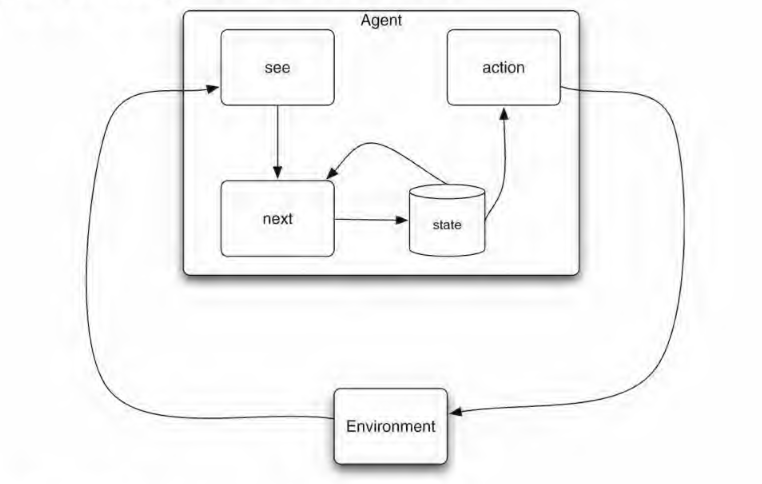
\includegraphics[width=500pt]{agent_with_state}
      \caption{Agent with state.}
      \label{StateAgent}
      \end{center}
    \end{figure}
\end{itemize}
Besides this architectures, there are also less formal and more human-like approaches.
One of them is called BDI (Belief-Desire-Intention) execution model \cite{DUMMY:1}.
BDI architecture uses terms from a folk psychology to describe the agent's behavioral structure. The 4 key concepts of this model are Belief, Desire, Intention and Plan (see Fig.\ref{BDIAgent}). Beliefs represent the agent's internal state. Desires are used by the reasoner (logical part of the agent) to determine the optimal course of actions. Intentions consist of actions that are going to be executed by the agent in order for it to achieve some of its desires. And, finally, plans can be described as long-term composite structures, that encapsulate an enumerated set of actions (intentions), used to simplify the belief system \cite[p.~150]{DUMMY:2}.
    \begin{figure}[h!]
      \begin{center}
      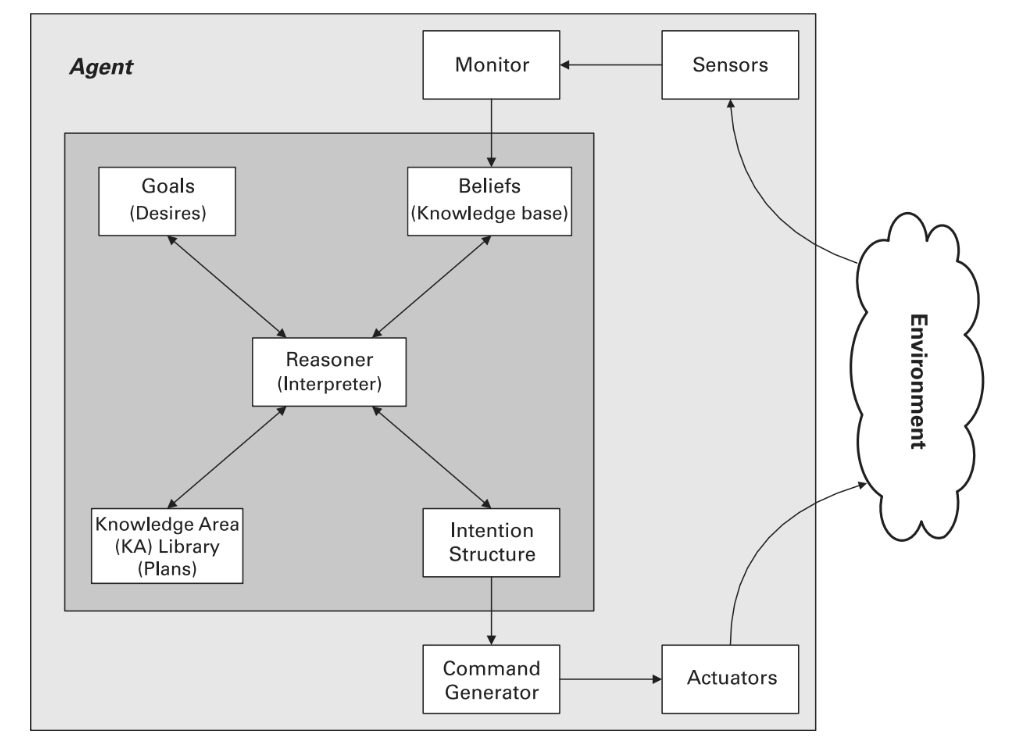
\includegraphics[width=400pt]{BDI}
      \caption{BDI agent architecture.}
      \label{BDIAgent}
      \end{center}
    \end{figure}

